% ============================================================
%  GÊMEO DIGITAL DE SEGURANÇA — Relatório Técnico Completo
%  Compilar com:  xelatex relatorio.tex  (2x para refs)
%  Apenas pacotes instalados no MiKTeX local (sem internet)
% ============================================================
\documentclass[a4paper,11pt]{article}

% ── Encoding & Fonts ────────────────────────────────────────
\usepackage{fontspec}
\setmainfont{Arial}[
  BoldFont       = {Arial Bold},
  ItalicFont     = {Arial Italic},
  BoldItalicFont = {Arial Bold Italic}
]
\setmonofont{Courier New}

% ── Layout (manual — sem geometry) ──────────────────────────
\setlength{\oddsidemargin}{0.5cm}
\setlength{\evensidemargin}{0.5cm}
\setlength{\textwidth}{16cm}
\setlength{\topmargin}{-1cm}
\setlength{\headheight}{1.2cm}
\setlength{\headsep}{0.5cm}
\setlength{\textheight}{23.5cm}
\setlength{\parindent}{0pt}
\setlength{\parskip}{6pt}

% ── Colors ──────────────────────────────────────────────────
\usepackage[dvipsnames]{xcolor}
\definecolor{blue1}{HTML}{1D4ED8}
\definecolor{blue2}{HTML}{2563EB}
\definecolor{blue3}{HTML}{DBEAFE}
\definecolor{darkbg}{HTML}{0F172A}
\definecolor{panelbg}{HTML}{1E293B}
\definecolor{red1}{HTML}{DC2626}
\definecolor{amber1}{HTML}{D97706}
\definecolor{green1}{HTML}{059669}
\definecolor{gray1}{HTML}{64748B}
\definecolor{gray2}{HTML}{F1F5F9}
\definecolor{codebg}{HTML}{1E293B}
\definecolor{codefg}{HTML}{E2E8F0}
\definecolor{hdr}{HTML}{1E40AF}

% ── Tables ──────────────────────────────────────────────────
\usepackage{booktabs}
\usepackage{tabularx}
\usepackage{longtable}
\usepackage{array}
\usepackage{multirow}
% thead helper (sem makecell)
\newcommand{\thead}[1]{\textbf{\color{blue1}#1}}

% ── Graphics & TikZ ─────────────────────────────────────────
\usepackage{graphicx}
\usepackage{tikz}
\usetikzlibrary{shapes.geometric, arrows.meta, fit,
                positioning, backgrounds, calc}

% ── Math ────────────────────────────────────────────────────
\usepackage{amsmath, amssymb}

% ── Code blocks ─────────────────────────────────────────────
\usepackage{listings}
\lstset{
  backgroundcolor=\color{codebg},
  basicstyle=\ttfamily\small\color{codefg},
  breaklines=true,
  frame=single,
  framesep=6pt,
  rulecolor=\color{blue2},
  keywordstyle=\color{cyan!80},
  stringstyle=\color{green!70},
  commentstyle=\color{gray1},
  showstringspaces=false,
  xleftmargin=10pt, xrightmargin=10pt,
  aboveskip=8pt, belowskip=8pt
}

% ── Hyperlinks ──────────────────────────────────────────────
% hyperref removido (kvsetkeys nao instalavel via mpm)

% ── Headers (sem fancyhdr — usa pagestyle myheadings) ───────
\makeatletter
\def\ps@myheadings{%
  \def\@oddhead{\small\color{gray1}Gêmeo Digital de Segurança AMR\hfill Hackathon Ericsson 2026}
  \def\@evenhead{\small\color{gray1}Gêmeo Digital de Segurança AMR\hfill Hackathon Ericsson 2026}
  \def\@oddfoot{\hfill\small\color{gray1}\thepage\hfill}
  \def\@evenfoot{\hfill\small\color{gray1}\thepage\hfill}
}
\makeatother

% ── Section styling (sem titlesec) ──────────────────────────
\makeatletter
\renewcommand{\section}{\@startsection{section}{1}{\z@}%
  {-18pt \@plus -4pt \@minus -2pt}%
  {8pt \@plus 2pt}%
  {\Large\bfseries\color{blue1}}}
\renewcommand{\subsection}{\@startsection{subsection}{2}{\z@}%
  {-12pt \@plus -2pt \@minus -1pt}%
  {4pt \@plus 1pt}%
  {\normalsize\bfseries\color{blue1}}}
\makeatother

% section rule
\let\oldsection\section
\renewcommand{\section}[1]{%
  \oldsection{#1}\nopagebreak\vspace{-10pt}%
  {\color{blue2}\rule{\linewidth}{1.5pt}}\vspace{4pt}}

% ── tcolorbox (instalado) ───────────────────────────────────
\usepackage{tcolorbox}
\tcbuselibrary{breakable}

% ── Helpers ─────────────────────────────────────────────────
\newcommand{\badge}[2]{%
  \colorbox{#1}{\color{white}\textbf{\footnotesize\ #2\ }}}
\newcommand{\alta}{\badge{red1}{ALTA}}
\newcommand{\med}{\badge{amber1}{MED}}
\newcommand{\baixa}{\badge{green1}{BAIXA}}
\newcommand{\ok}{\badge{gray1}{OK}}

% ============================================================
\begin{document}
\thispagestyle{empty}

% ──────────────────────────────────────────────────────────
%  CAPA
% ──────────────────────────────────────────────────────────
\begin{tikzpicture}[remember picture, overlay]
  \fill[darkbg] (current page.south west) rectangle (current page.north east);
  \fill[blue1, opacity=0.15]
    (current page.south west) rectangle
    ([yshift=5cm]current page.south east);
  \draw[blue2, line width=3pt]
    ([xshift=2.5cm, yshift=-3.5cm]current page.north west) --
    ([xshift=-2.5cm,yshift=-3.5cm]current page.north east);
  \draw[blue2, line width=3pt]
    ([xshift=2.5cm, yshift=2.5cm]current page.south west) --
    ([xshift=-2.5cm,yshift=2.5cm]current page.south east);
\end{tikzpicture}

\vspace*{3.5cm}
\begin{center}
  {\fontsize{36}{44}\selectfont\bfseries\color{white}
    GÊMEO DIGITAL\par}
  {\fontsize{18}{22}\selectfont\color{blue3}
    DE SEGURANÇA INDUSTRIAL\par}
  \vspace{0.4cm}
  {\large\color{gray1} AMR Fire Detection\ ·\ Command Center 3D\,/\,VR}

  \vspace{2cm}
  \begin{tikzpicture}
    \node[fill=panelbg, draw=blue2, rounded corners=8pt,
          inner xsep=18pt, inner ysep=12pt, line width=1.2pt] {
      \color{white}
      \begin{tabular}{@{}l@{\hspace{18pt}}l@{}}
        \color{blue3}\textbf{Projeto}    & Gêmeo Digital de Segurança Industrial \\[4pt]
        \color{blue3}\textbf{Evento}     & Hackathon Ericsson 2026 \\[4pt]
        \color{blue3}\textbf{Data}       & 06 de Maio de 2026 \\[4pt]
        \color{blue3}\textbf{Stack}      & Python\ ·\ Node.js\ ·\ React 18\ ·\ Three.js\ ·\ WebXR \\[4pt]
        \color{blue3}\textbf{Modelo IA}  & YOLOv8/12 (fire / smoke detection) \\[4pt]
        \color{blue3}\textbf{Repositório} & \texttt{C:/GEMEODIGITAL/} \\
      \end{tabular}
    };
  \end{tikzpicture}

  \vspace{2.4cm}
  {\LARGE\bfseries\color{white} Relatório Técnico Completo}
\end{center}

\vspace*{\fill}
\begin{center}
  \color{gray1}\small Documento gerado em 06/05/2026\ ·\ Hackathon Ericsson 2026
\end{center}

\newpage
\pagestyle{myheadings}
\setcounter{page}{1}

% ──────────────────────────────────────────────────────────
%  SUMÁRIO EXECUTIVO
% ──────────────────────────────────────────────────────────
\begin{tcolorbox}[
  colback=blue3, colframe=blue1,
  title={\textbf{Resumo Executivo}},
  fonttitle=\bfseries\color{white},
  colbacktitle=blue1,
  sharp corners=south, rounded corners=north,
  boxrule=0.8pt, left=8pt, right=8pt, top=6pt, bottom=6pt
]
Este documento descreve a arquitetura técnica, as implementações concluídas e as
pendências de cada squad do sistema \textbf{Gêmeo Digital de Segurança Industrial}.
O sistema integra visão computacional por IA (YOLO), backend em tempo real
(Node.js + WebSocket) e uma interface 3D/VR imersiva (React Three Fiber) para
monitoramento de um robô AMR em uma usina térmica, com localização por otimização
matemática (Lagrange + Gradiente) e verificação de consistência com relatórios LLM.
\end{tcolorbox}

\tableofcontents
\newpage

% ============================================================
\section{Arquitetura do Sistema}
% ============================================================

O sistema é composto por \textbf{três camadas independentes} que comunicam via
contratos de dados JSON bem definidos. Cada camada pode ser desenvolvida, testada
e substituída de forma isolada.

\subsection{Mapa de Arquitetura}

\begin{figure}[h!]
\centering
\begin{tikzpicture}[
  node distance = 1.4cm,
  layer/.style  = {draw=blue2, fill=panelbg, text=white, rounded corners=6pt,
                   minimum width=4cm, minimum height=0.7cm, font=\small\bfseries,
                   inner sep=6pt, line width=1pt},
  sub/.style    = {draw=blue2!50, fill=darkbg, text=codefg, rounded corners=4pt,
                   minimum width=3.2cm, minimum height=0.55cm, font=\footnotesize,
                   inner sep=5pt, line width=0.6pt},
  arr/.style    = {->, thick, color=blue2!80},
  bg/.style     = {rounded corners=8pt, inner sep=10pt}
]

% ── EDGE ────────────────────────────────────────────────
\node[layer, fill=red1!70!black] (edge) {[1] EDGE — Python};
\node[sub, below=0.3cm of edge]        (e1)  {fire\_equipe2.py};
\node[sub, below=0.2cm of e1]          (e2)  {best.pt — YOLOv8};
\node[sub, below=0.2cm of e2]          (e3)  {Heartbeat 3\,s};
\node[sub, below=0.2cm of e3]          (e4)  {PATROL\_PATH × 4};

% ── BACKEND ─────────────────────────────────────────────
\node[layer, fill=amber1!70!black, right=3.5cm of edge] (bk) {[2] BACKEND — Node.js};
\node[sub, below=0.3cm of bk]          (b1)  {server.js :3000};
\node[sub, below=0.2cm of b1]          (b2)  {WebSocket :3001};
\node[sub, below=0.2cm of b2]          (b3)  {POST /alerta};
\node[sub, below=0.2cm of b3]          (b4)  {LLM Report (mock)};

% ── FRONTEND ────────────────────────────────────────────
\node[layer, fill=green1!70!black,
      below=2.2cm of $(edge)!0.5!(bk)$] (fe) {[3] FRONTEND — React + Three.js};
\node[sub, below=0.3cm of fe]           (f1)  {DashboardAMR.jsx};
\node[sub, below=0.2cm of f1]           (f2)  {3D Canvas / VR};
\node[sub, below=0.2cm of f2]           (f3)  {Lerp + Lagrange};
\node[sub, below=0.2cm of f3]           (f4)  {WS :3001};

% ── ARROWS ──────────────────────────────────────────────
\draw[arr] (e4.south) -- ++(0,-0.3) -| ($(fe.north) + (-1,0)$)
           node[midway, left, font=\tiny, text=gray1] {POST /alerta :3000};
\draw[arr] (b4.south) -- ++(0,-0.3) -| ($(fe.north) + (1,0)$)
           node[midway, right, font=\tiny, text=gray1] {WS broadcast :3001};
\draw[arr] (edge.east) -- (bk.west)
           node[midway, above, font=\tiny, text=gray1] {HTTP POST};

\end{tikzpicture}
\caption{Arquitetura de 3 camadas — fluxo entre squads}
\end{figure}

\subsection{Responsabilidades por Camada}

\begin{tabularx}{\linewidth}{@{}>{\bfseries\color{blue1}}l X X@{}}
\thead{Camada} & \thead{Tecnologia} & \thead{Responsabilidade Principal} \\
\midrule
Edge / IA  & Python 3.10 + YOLOv8/12        & Inferência em tempo real, heartbeat de patrulha a cada 3\,s \\
Backend    & Node.js + Express + WebSocket   & Validação do contrato JSON, geração de relatório LLM, broadcast WS \\
Frontend   & React 18 + Three.js + WebXR     & Dashboard 3D/VR, robô animado por lerp, verificação Lagrange \\
\bottomrule
\end{tabularx}

\subsection{Pipeline de Dados}

\begin{figure}[h!]
\centering
\begin{tikzpicture}[
  box/.style  = {draw=blue2, fill=panelbg, text=white, rounded corners=4pt,
                 minimum width=2.1cm, minimum height=1.1cm, align=center,
                 font=\footnotesize\bfseries, inner sep=5pt, line width=0.8pt},
  sub/.style  = {font=\tiny, text=gray1},
  arr/.style  = {->, thick, color=blue2!70},
  node distance = 0.3cm
]
\node[box]                           (cam)  {CÂMARA\\AMR};
\node[box, right=0.8cm of cam]       (yolo) {YOLO\\INFERÊNCIA};
\node[box, right=0.8cm of yolo]      (post) {POST\\{\small/alerta}};
\node[box, right=0.8cm of post]      (node) {NODE.JS\\BACKEND};
\node[box, right=0.8cm of node]      (ws)   {WS\\BROADCAST};
\node[box, right=0.8cm of ws]        (dash) {REACT\\DASHBOARD};
\node[box, right=0.8cm of dash]      (view) {3D / VR\\VIEW};

\foreach \a/\b in {cam/yolo, yolo/post, post/node, node/ws, ws/dash, dash/view}
  \draw[arr] (\a.east) -- (\b.west);

\node[sub, below=0.15cm of cam]  {videoCapture(0)};
\node[sub, below=0.15cm of yolo] {CONF\_FRAMES≥5};
\node[sub, below=0.15cm of post] {HTTP :3000};
\node[sub, below=0.15cm of node] {Valida + LLM};
\node[sub, below=0.15cm of ws]   {ws://\,:\,3001};
\node[sub, below=0.15cm of dash] {lerp + Lagrange};
\node[sub, below=0.15cm of view] {Three.js/XR};

\node[below=1cm of $(post)!0.5!(node)$, font=\small, text=gray1]
  {Latência estimada ponta-a-ponta: $<\,1{,}5$\,s \quad (câmara\,$\to$\,dashboard)};
\end{tikzpicture}
\caption{Pipeline ponta-a-ponta: câmara $\to$ YOLO $\to$ backend $\to$ WS $\to$ Three.js}
\end{figure}

\subsection{Contrato JSON — POST /alerta}

\begin{lstlisting}[language={}]
{
  "id_alerta"           : "ALRT-1234",
  "timestamp"           : "2026-05-06T19:40:00Z",
  "evento"              : "fogo | fumaca | normal",
  "confianca"           : 0.94,
  "localizacao_otimizada": {
    "x"    : 350,
    "y"    : 120,
    "setor": "Setor D - Caldeiras Quimicas"
  },
  "llm_prompt": "URGENTE: fogo no Setor D..."
}
\end{lstlisting}

O campo \texttt{localizacao\_otimizada.setor} é mapeado para coordenadas 3D pelo
frontend via \texttt{SECTOR\_TO\_3D}.

\newpage
% ============================================================
\section{Modelo Matemático — Localização por Otimização}
% ============================================================

A localização precisa do AMR na planta 3D é resolvida por \textbf{cinco blocos
matemáticos} complementares, todos executados em tempo real no frontend
(60\,fps via \texttt{useFrame}):

\subsection{Mapa Mental do Modelo}

\begin{figure}[h!]
\centering
\begin{tikzpicture}[
  center/.style  = {circle, fill=blue1, text=white, font=\footnotesize\bfseries,
                    minimum size=1.8cm, align=center, line width=0},
  block/.style   = {draw=#1!80, fill=#1!20!darkbg, text=white,
                    rounded corners=5pt, minimum width=3.6cm,
                    minimum height=1.8cm, align=center,
                    font=\footnotesize, inner sep=6pt, line width=1pt},
  arr/.style     = {<->, thick, color=blue2!60}
]
\node[center] (C) {LOCALIZAÇÃO\\DO AMR};

\node[block=red1,    above left  = 1.8cm and 2.8cm of C] (B1)
  {\textbf{(1) Função de Custo}\\[3pt]
   $J(x,z)=\sum_i(d_i - r_i)^2$\\
   $d_i=\sqrt{(x-a_{xi})^2+(z-a_{zi})^2}$\\[2pt]
   \textit{Trilateration}};

\node[block=amber1,  above right = 1.8cm and 2.8cm of C] (B2)
  {\textbf{(2) Lagrange}\\[3pt]
   $\min\|p - p_{\text{target}}\|^2$\\
   s.t.\ $p \in \overline{W_k W_{k+1}}$\\
   $t^* = \mathrm{clamp}\!\left(\frac{(p-W_k)\cdot d}{|d|^2},0,1\right)$};

\node[block=green1,  below left  = 1.8cm and 2.8cm of C] (B3)
  {\textbf{(3) Gradient Descent}\\[3pt]
   $p(t+\Delta t)=p(t)+\alpha(p_T - p(t))$\\
   $\alpha = \text{SPEED}\cdot\Delta t\,/\,\text{dist}$\\[2pt]
   \texttt{lerp} 2\,m/s — sem teleporte};

\node[block=blue2,   below right = 1.8cm and 2.8cm of C] (B4)
  {\textbf{(4) Consistência LLM}\\[3pt]
   $\text{conf}=e^{-\beta\|p^*-C_s\|^2}$\\
   $\beta=0{,}18$\ \ threshold\,$=0{,}60$\\[2pt]
   \checkmark verde\ /\ $\times$ vermelho HUD};

\node[block=purple!80,  below = 2.2cm of C] (B5)
  {\textbf{(5) Orientação do Robô}\\[3pt]
   $\theta = \mathrm{atan2}(\Delta x,\,\Delta z)$\\
   $\theta_c = \mathrm{lerp}(\theta_c,\,\theta,\,8\Delta t)$\\[2pt]
   \texttt{group.rotation.y}};

\foreach \b in {B1,B2,B3,B4,B5}
  \draw[arr] (C) -- (\b);
\end{tikzpicture}
\caption{Mapa mental do modelo matemático de localização do AMR}
\end{figure}

\subsection{Equações Principais}

\begin{tabularx}{\linewidth}{@{}>{\bfseries}p{3.6cm} p{5.8cm} X@{}}
\thead{Módulo} & \thead{Equação Central} & \thead{Implementação no Código} \\
\midrule
\textnumero1 Função de Custo (Trilateration) &
  $J(x,z)=\sum_i(d_i-r_i)^2$,\; $d_i=\sqrt{(x{-}a_{xi})^2+(z{-}a_{zi})^2}$ &
  Base para estimar posição por múltiplos âncoras LIDAR \\

\textnumero2 Gradient Descent (lerp) &
  $p(t{+}\Delta t) = p(t) + \alpha(p_T - p(t))$,\; $\alpha = \text{SPEED}\cdot\Delta t\,/\,\text{dist}$ &
  \texttt{useFrame()}: lerp adaptativo 2\,m/s — sem teleporte \\

\textnumero3 Lagrange (path constraint) &
  $\min\|p-p_T\|^2$ s.t. $p\in\overline{W_k W_{k+1}}$,\;
  $t^*=\mathrm{clamp}\!\left(\tfrac{(p-W_k)\cdot d}{|d|^2},0,1\right)$ &
  \texttt{projectOntoPatrolPath()} — solução fechada $O(n_{\text{seg}})$ \\

\textnumero4 Consistência LLM$\leftrightarrow$Física &
  $\mathrm{conf}=e^{-\beta\|p^*-C_s\|^2}$,\; $\beta=0{,}18$, threshold\,$=0{,}60$ &
  \texttt{computeLocationConsistency()} — \checkmark/\texttimes\ no HUD \\

\textnumero5 Orientação do Robô &
  $\theta=\mathrm{atan2}(\Delta x,\Delta z)$,\;
  $\theta_c=\mathrm{lerp}(\theta_c,\theta,8\Delta t)$ &
  \texttt{group.rotation.y} — visor aponta para destino \\
\bottomrule
\end{tabularx}

\subsection{Mapeamento Setores $\to$ Coordenadas 3D}

\begin{tabularx}{\linewidth}{@{}X c c c l@{}}
\thead{Setor (texto LLM)} & \thead{x3d} & \thead{y3d} & \thead{z3d} & \thead{THREE.Vector3} \\
\midrule
Setor A — Turbinas            & $-4$ & $0.5$ & $-3$ & \texttt{Vector3(-4,\;0.5,\;-3)} \\
Setor B — Geradores           & $+4$ & $0.5$ & $-3$ & \texttt{Vector3(+4,\;0.5,\;-3)} \\
Setor C — Painéis de Controle & $-4$ & $0.5$ & $+3$ & \texttt{Vector3(-4,\;0.5,\;+3)} \\
Setor D — Caldeiras Químicas  & $+4$ & $0.5$ & $+3$ & \texttt{Vector3(+4,\;0.5,\;+3)} \\
\bottomrule
\end{tabularx}

\newpage
% ============================================================
\section{Estado Atual — O que está Implementado}
% ============================================================

\begin{longtable}{@{}>{\small}p{4.6cm} >{\small}c >{\small\ttfamily}p{3.4cm} >{\small}X@{}}
\textbf{\color{white}Funcionalidade} &
\textbf{\color{white}Camada} &
\textbf{\color{white}Ficheiro} &
\textbf{\color{white}Detalhe Técnico} \\
\endfirsthead
\textbf{\color{white}Funcionalidade} &
\textbf{\color{white}Camada} &
\textbf{\color{white}Ficheiro} &
\textbf{\color{white}Detalhe Técnico} \\
\endhead
\midrule
3D Canvas com GLB da usina
  & Frontend & DashboardAMR.jsx
  & \texttt{usina\_interno.glb} carregado via \texttt{useGLTF} + Suspense \\
RobotAMR mesh 3D completo
  & Frontend & DashboardAMR.jsx
  & Chassis, cabine, visor, 4 rodas, LIDAR cilíndrico, antena \\
Movimento suave (lerp)
  & Frontend & DashboardAMR.jsx
  & Gradient descent 2\,m/s por frame — sem teleporte \\
Rotação do robô
  & Frontend & DashboardAMR.jsx
  & atan2 + lerp angular — visor aponta sempre para destino \\
Rodas animadas
  & Frontend & DashboardAMR.jsx
  & \texttt{rotation.x += 4·$\Delta$t} quando distância ao alvo $>0.05$ \\
Projeção Lagrangiana no caminho
  & Frontend & DashboardAMR.jsx
  & \texttt{projectOntoPatrolPath()} — solução fechada $O(n_{\text{seg}})$ \\
Verificação LLM $\leftrightarrow$ posição
  & Frontend & DashboardAMR.jsx
  & Gaussiana $\mathrm{conf}=e^{-0.18d^2}$, exibida no HUD \\
Indicador CONF.\,POS no HUD
  & Frontend & DashboardAMR.jsx
  & \checkmark verde $\geq60\%$, $\times$ vermelho $<60\%$ \\
Badge LIVE / DEMO
  & Frontend & DashboardAMR.jsx
  & Verde = WebSocket ativo, Amarelo = fallback mock \\
Modo VR — WebXR
  & Frontend & DashboardAMR.jsx
  & \texttt{@react-three/xr} — botão ENTRAR VR, suporta Quest \\
Grid tático 3D
  & Frontend & DashboardAMR.jsx
  & Linhas de referência + secções $4{\times}4$ na cena \\
WebSocket + reconexão auto
  & Frontend & DashboardAMR.jsx
  & Reconecta a cada 5\,s se WS cair \\
Mock fallback (sem backend)
  & Frontend & DashboardAMR.jsx
  & Simula patrulha A$\to$B$\to$D$\to$C a cada 4\,s \\
\midrule
POST /alerta validado
  & Backend & server.js
  & Schema validation, enriquece + broadcast WS \\
LLM report (mock)
  & Backend & server.js
  & \texttt{generateLLMReport()} estruturado, pronto para API real \\
Histórico em memória
  & Backend & server.js
  & \texttt{GET /alertas} retorna últimas 50 entradas \\
GET /health
  & Backend & server.js
  & Clientes WS, uptime, total alertas \\
\midrule
Heartbeat de patrulha
  & Edge & fire\_equipe2.py
  & Envia evento \texttt{"normal"} + setor atual a cada 3\,s \\
PATROL\_PATH 4 setores
  & Edge & fire\_equipe2.py
  & Rota A$\to$B$\to$D$\to$C em loop (substituível por GPS) \\
Filtro temporal YOLO
  & Edge & fire\_equipe2.py
  & \texttt{CONFIRMATION\_FRAMES=5} — anti-falso-positivo \\
Fallback yolov8n
  & Edge & download\_model.py
  & Pipeline funciona completo sem \texttt{best.pt} Squad 1 \\
\midrule
Reestruturação de pastas
  & Infra & edge/models/
  & \texttt{yolov8n} movido para \texttt{edge/models/}, \texttt{styles/} removido \\
\bottomrule
\end{longtable}

\newpage
% ============================================================
\section{Sprint Final — O que falta por Squad}
% ============================================================

\subsection{Mapa de Pendências}

\begin{figure}[h!]
\centering
\begin{tikzpicture}[
  squad/.style  = {draw=#1, fill=#1!15!darkbg, text=white,
                   rounded corners=6pt, minimum width=5.2cm,
                   minimum height=0.7cm, align=center,
                   font=\small\bfseries, inner sep=7pt, line width=1.2pt},
  item/.style   = {draw=#1!60, fill=#1!10!darkbg, text=white,
                   rounded corners=3pt, minimum width=5cm,
                   minimum height=0.52cm, align=left,
                   font=\footnotesize, inner sep=5pt, line width=0.6pt},
  done/.style   = {draw=gray1!60, fill=gray1!15!darkbg, text=gray1,
                   rounded corners=3pt, minimum width=5cm,
                   minimum height=0.52cm, align=left,
                   font=\footnotesize, inner sep=5pt, line width=0.5pt},
  node distance = 0.22cm
]
% Squad 1 — EDGE (top-left)
\node[squad=red1]                             (s1)  {[1] SQUAD 1 — EDGE / IA};
\node[item=red1,   below=0.3cm of s1]         (s1a) {[ALTA] Stream RTSP câmara AMR};
\node[item=red1,   below=0.2cm of s1a]        (s1b) {[ALTA] GPS / odometria real};
\node[item=amber1, below=0.2cm of s1b]        (s1c) {[MED]  Validar classes best.pt};
\node[item=amber1, below=0.2cm of s1c]        (s1d) {[MED]  PATROL\_PATH dinâmico (API)};
\node[item=green1, below=0.2cm of s1d]        (s1e) {[LOW]  Log de deteções em disco};

% Squad 2 — BACKEND (top-right)
\node[squad=amber1, right=3cm of s1]          (s2)  {[2] SQUAD 2 — BACKEND};
\node[item=red1,   below=0.3cm of s2]         (s2a) {[ALTA] Integrar LLM real (OpenAI/Ollama)};
\node[item=red1,   below=0.2cm of s2a]        (s2b) {[ALTA] Persistência SQLite/JSON};
\node[item=amber1, below=0.2cm of s2b]        (s2c) {[MED]  Autenticação X-AMR-Token};
\node[item=amber1, below=0.2cm of s2c]        (s2d) {[MED]  Rate limiting express};
\node[item=green1, below=0.2cm of s2d]        (s2e) {[LOW]  Endpoint GET /stats};

% Squad 3 — FRONTEND (bottom-right)
\node[squad=green1, below=1.8cm of s2e]       (s3)  {[3] SQUAD 3 — FRONTEND};
\node[item=red1,   below=0.3cm of s3]         (s3a) {[ALTA] Calibrar coords 3D vs GLB};
\node[item=red1,   below=0.2cm of s3a]        (s3b) {[ALTA] Feed vídeo real (MJPEG/WS)};
\node[item=red1,   below=0.2cm of s3b]        (s3c) {[ALTA] Painel histórico alertas};
\node[item=amber1, below=0.2cm of s3c]        (s3d) {[MED]  Botão "Acionar Brigada"};
\node[item=green1, below=0.2cm of s3d]        (s3e) {[LOW]  Alarme sonoro};

% Concluído (bottom-left)
\node[squad=gray1, below=1.8cm of s1e]        (ok)  {[OK] CONCLUÍDO};
\node[done, below=0.3cm of ok]                (d1)  {[OK] 3D Canvas + GLB usina};
\node[done, below=0.2cm of d1]                (d2)  {[OK] RobotAMR mesh 3D completo};
\node[done, below=0.2cm of d2]                (d3)  {[OK] WebSocket + mock fallback};
\node[done, below=0.2cm of d3]                (d4)  {[OK] Lagrange + verificação LLM};
\node[done, below=0.2cm of d4]                (d5)  {[OK] Heartbeat patrulha 3\,s};

% Central label
\node[fill=blue1, text=white, rounded corners=5pt, font=\small\bfseries,
      inner sep=8pt,
      at={($(s1)!0.5!(s2) + (0,-3.5)$)}]     (hub) {SPRINT FINAL};

\end{tikzpicture}
\caption{Mapa de pendências por squad}
\end{figure}

\subsection{Squad 1 — Edge / IA (Python)}

\begin{tabularx}{\linewidth}{@{}>{\centering\arraybackslash}p{1.5cm} p{4.2cm} X >{\centering\arraybackslash}p{1.2cm}@{}}
\thead{Prior.} & \thead{Tarefa} & \thead{Descrição Técnica} & \thead{Est.} \\
\midrule
\alta  & Stream RTSP câmara     & Trocar \texttt{VideoCapture(0)} por \texttt{rtsp://IP\_AMR/stream}           & 2\,h \\
\alta  & GPS/odometria real     & \texttt{PATROL\_PATH} via MQTT/Serial da telemetria do AMR                   & 4\,h \\
\med   & Validar best.pt        & Confirmar classes \{0:smoke, 1:fire\} no modelo Squad 1                      & 1\,h \\
\med   & PATROL\_PATH dinâmico  & Receber posição do AMR por API em tempo real                                 & 3\,h \\
\baixa & Log de deteções        & Guardar frames com deteções em disco para auditoria                          & 1\,h \\
\bottomrule
\end{tabularx}

\subsection{Squad 2 — Backend (Node.js)}

\begin{tabularx}{\linewidth}{@{}>{\centering\arraybackslash}p{1.5cm} p{4.2cm} X >{\centering\arraybackslash}p{1.2cm}@{}}
\thead{Prior.} & \thead{Tarefa} & \thead{Descrição Técnica} & \thead{Est.} \\
\midrule
\alta  & LLM real              & Substituir \texttt{generateLLMReport()} por OpenAI/Ollama API & 3\,h \\
\alta  & Persistência          & \texttt{better-sqlite3} ou ficheiro JSON append-only          & 2\,h \\
\med   & Autenticação          & Header \texttt{X-AMR-Token} fixo no \texttt{POST /alerta}     & 1\,h \\
\med   & Rate limiting         & \texttt{express-rate-limit} — máx 10 req/min por IP           & 0.5\,h \\
\baixa & Endpoint métricas     & \texttt{GET /stats} com contagem por evento e intervalo       & 1\,h \\
\bottomrule
\end{tabularx}

\subsection{Squad 3 — Frontend (React + Three.js)}

\begin{tabularx}{\linewidth}{@{}>{\centering\arraybackslash}p{1.5cm} p{4.2cm} X >{\centering\arraybackslash}p{1.2cm}@{}}
\thead{Prior.} & \thead{Tarefa} & \thead{Descrição Técnica} & \thead{Est.} \\
\midrule
\alta  & Calibrar coords 3D    & Alinhar \texttt{SECTOR\_TO\_3D} com geometria real do GLB (Blender) & 2\,h \\
\alta  & Feed vídeo real       & \texttt{<video>} MJPEG ou WebRTC substituindo o CSS placeholder      & 3\,h \\
\alta  & Histórico alertas     & Painel lateral consumindo \texttt{GET /alertas} + filtros           & 2\,h \\
\med   & Botão "Acionar Brigada" & POST para webhook Slack/Teams/e-mail                            & 1\,h \\
\med   & Alarme sonoro         & \texttt{new Audio("alarm.mp3").play()} em \texttt{isAlert → true} & 0.5\,h \\
\baixa & Snapshot PDF          & Botão para exportar estado atual como PDF                           & 2\,h \\
\bottomrule
\end{tabularx}

\newpage
% ============================================================
\section{Como Rodar o Sistema}
% ============================================================

\begin{tabularx}{\linewidth}{@{}>{\bfseries\small}p{2.4cm} >{\ttfamily\small}p{5.2cm} X@{}}
\thead{Passo} & \thead{Comando} & \thead{Resultado Esperado} \\
\midrule
1. Deps Node    & npm install                           & Instala React, Three.js, Express, WS, Vite \\
2. Deps Python  & pip install -r edge/requirements.txt  & Instala ultralytics, opencv-python, requests \\
3. Modelo IA    & python edge/download\_model.py        & Cria \texttt{edge/models/best.pt} (ou fallback COCO) \\
4. Tudo junto   & npm start                             & Backend :3000/:3001 + Frontend :5173 \\
5. Dashboard    & http://localhost:5173                 & Interface 3D/VR — badge DEMO até Python ligar \\
6. Câmara IA    & python -m edge.fire\_equipe2          & YOLO + heartbeat 3\,s → badge muda para LIVE \\
7. Testar alerta & (curl/Postman — test\_payload.json)  & Robô vai para Setor D e entra em modo ALERT \\
\bottomrule
\end{tabularx}

\subsection{Portas e Serviços}

\begin{tabularx}{\linewidth}{@{}>{\ttfamily\bfseries}c >{\bfseries}c X l@{}}
\thead{Porta} & \thead{Protocolo} & \thead{Serviço} & \thead{Consumido por} \\
\midrule
3000 & HTTP      & Express API (POST /alerta · GET /alertas · GET /health) & \texttt{fire\_equipe2.py} \\
3001 & WebSocket & Broadcast de telemetria em tempo real                   & \texttt{DashboardAMR.jsx} \\
5173 & HTTP      & Vite Dev Server — React + Three.js                      & Browser do operador \\
0    & V4L2/DShow & VideoCapture — webcam local ou stream RTSP              & \texttt{fire\_equipe2.py} \\
\bottomrule
\end{tabularx}

\vspace{1.5cm}
\begin{center}
\begin{tikzpicture}
  \node[fill=darkbg, draw=blue2, rounded corners=6pt,
        inner xsep=20pt, inner ysep=10pt, line width=1pt] {
    \color{gray1}\small
    Documento gerado automaticamente em 06/05/2026
    \quad\textbf{\color{blue2}·}\quad
    Hackathon Ericsson 2026
  };
\end{tikzpicture}
\end{center}

\end{document}


